\begin{frame}
    \frametitle{Representación de pose en 2D}
    \footnotesize
    Modelamos el robot como un cuerpo rígido sobre ruedas, que opera en un plano horizontal. La dimensionalidad total de este chasis de robot en el plano es de 3: 2 para la posición en el plano y 1 para la orientación a lo largo del eje vertical, que es ortogonal al plano.

    \begin{figure}[!h]
        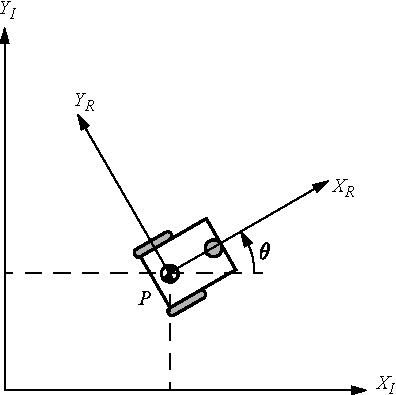
\includegraphics[width=0.3\columnwidth]{./images/coordinate_systems.pdf}
        \caption{El marco de referencia global y el marco de referencia local del robot.}
    \end{figure}

    Para especificar la posición del robot en el plano, establecemos una relación entre el {\bf marco de referencia global} y el {\bf marco de referencia local del robot}.

\end{frame}


\begin{frame}
    \frametitle{Representación de pose en 2D}
    \footnotesize

    \begin{figure}
        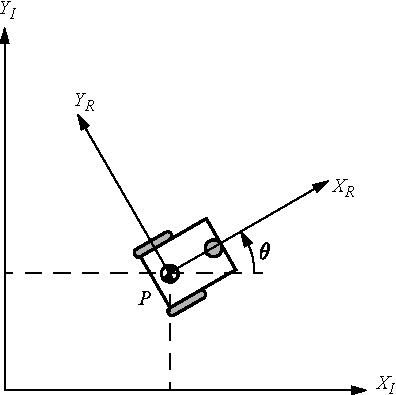
\includegraphics[width=0.3\columnwidth]{./images/coordinate_systems.pdf}
    \end{figure}

    \note{Un marco de referencia inercial es un marco de referencia que no está experimentando aceleración. La física de un sistema en un marco inercial no tiene fuerzas externas al sistema.}

    \note{Ejemplo de sistema no inercial: una bola que cae hacia el suelo no va exactamente hacia abajo porque la Tierra está girando, lo que significa que el marco de referencia de un observador en la Tierra no es inercial. La física debe tener en cuenta el efecto Coriolis, en este caso considerado como una fuerza, para predecir el movimiento horizontal.}

    Los ejes $X_I$ y $Y_I$ definen una {\bf base inercial} arbitraria en el plano como marco de referencia global de algún {\bf origen} $O:\left\lbrace X_I,Y_I \right\rbrace$.Para especificar la posición del robot, elegimos un punto $p$ en el chasis del robot como su punto de referencia de posición. La base $\left\lbrace X_R,Y_R \right\rbrace$ define dos ejes en relación con $p$ en el chasis del robot y, por lo tanto, es el {\bf marco de referencia local del robot}. La posición de $p$ en el {\bf marco de referencia global} se especifica mediante las coordenadas $x$ e $y$, y la diferencia angular entre los marcos de referencia global y local está dada por $\theta$.

\end{frame}


\begin{frame}
    \frametitle{Cinemática de un robot diferencial}

    \begin{figure}
        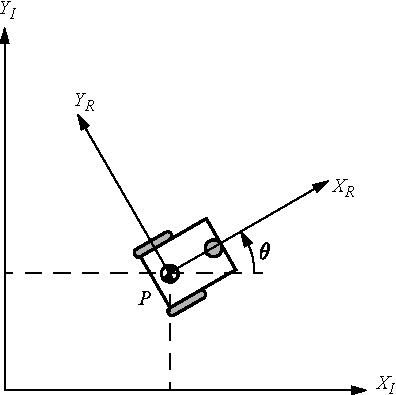
\includegraphics[width=0.3\columnwidth]{./images/coordinate_systems.pdf}
    \end{figure}

    La pose del robot estará dada por la posición y la orientación:

    \begin{equation*}
        \transform{I}{} =
        \begin{bmatrix}
            x\\
            y\\
            \theta
        \end{bmatrix}
    \end{equation*}
\end{frame}


\begin{frame}
    \frametitle{Cinemática de un robot diferencial}
    \small
    \begin{center}
        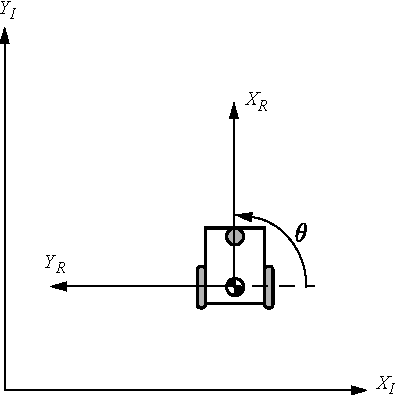
\includegraphics[width=0.2\columnwidth]{./images/coordinate_frame_rotation.pdf}
    \end{center}

    Para {\bf describir el movimiento del robot} en términos de movimientos de componentes, será necesario {\bf mapear el movimiento a lo largo de los ejes del marco de referencia global al movimiento a lo largo de los ejes del marco de referencia local del robot}. Por supuesto, el mapeo es una función de la pose actual del robot. Este mapeo se logra usando la matriz de rotación ortogonal:

    \begin{equation*}
    R(\theta)=
    \begin{bmatrix}
        \cos\theta & \sin\theta & 0\\
        -\sin \theta & \cos \theta & 0\\
        0 & 0 & 1
    \end{bmatrix}
\end{equation*}

    Esta matriz se puede utilizar para mapear el movimiento en el marco de referencia global $\left\lbrace X_I,Y_I \right\rbrace$ al movimiento en términos del marco de referencia local $\left\lbrace X_R,Y_R \right\rbrace$. Esta operación se denota por $R(\theta)\transform{I}{}$ · Porque el cálculo de esta operación depende del valor de $\theta$.
\end{frame}

\begin{frame}
    \frametitle{Cinemática de un robot diferencial}

    \begin{center}
        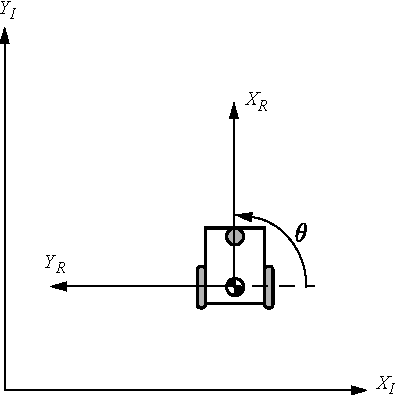
\includegraphics[width=0.2\columnwidth]{./images/coordinate_frame_rotation.pdf}
    \end{center}

    Dada alguna velocidad $(\dot{x}, \dot{y}, \dot{\theta})$ en el marco de referencia global, podemos calcular las componentes del movimiento a lo largo de los ejes locales $X_R$ y $Y_R$ del robot. En este caso, debido al ángulo específico del robot, el movimiento a lo largo de $X_R$ es igual a $\dot{y}$, y el movimiento a lo largo de $Y_R$ es $-\dot{x}$:

    \begin{equation*}
        \dot{\transform{R}{}} = R(\frac{\pi}{2})\dot{\transform{I}{}} =
        \begin{bmatrix}
            0 & 1 & 0 \\
            -1 & 0 & 0 \\
            0 & 0 & 1
        \end{bmatrix}
        \begin{bmatrix}
            \dot{x}\\
            \dot{y}\\
            \dot{\theta}
        \end{bmatrix}
         =
        \begin{bmatrix}
            \dot{y}\\
            -\dot{x}\\
            \dot{\theta}
        \end{bmatrix}
    \end{equation*}
\end{frame}

\begin{frame}
    \frametitle{Modelo de cinemática directa de un robot diferencial}
    \scriptsize
    \begin{figure}[!h]
        \centering
        \subfloat[]
        {
            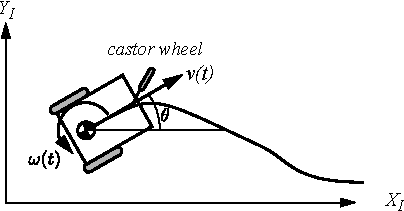
\includegraphics[width=0.3\columnwidth]{./images/differential_drive.pdf}
        }
        \subfloat[]
        {
            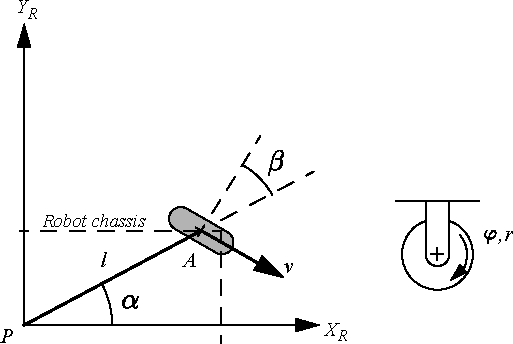
\includegraphics[width=0.25\columnwidth]{./images/wheel_parameters.pdf}
        }
    \end{figure}

    \begin{equation*}
        \dot{\transform{I}{}} =
        \begin{bmatrix}
            \dot{x}\\
            \dot{y}\\
            \dot{\theta}
        \end{bmatrix} =
        f\left( l,r,\theta,\dot{\varphi}_{1},\dot{\varphi}_{2}\right)
    \end{equation*}
    donde
    \begin{itemize}
        \item $r$ es el diámetro de las ruedas.
        \item $p$ es punto en el medio del eje de las ruedas
        \item $l$ es la distancia de cada rueda al punto $p$
        \item $\dot{\varphi}_{1}$ y $\dot{\varphi}_{2}$ la velocidad de giro de cada rueda
    \end{itemize}

    Podemos calcular el movimiento del robot en el marco de referencia global a partir del movimiento en su marco de referencia local:  $\dot{\transform{I}{}} = \inverse{R(\frac{\pi}{2})}\dot{\transform{R}{}}$. Por lo tanto, la estrategia será calcular primero la contribución de cada una de las dos ruedas en el marco de referencia local $\dot{\transform{R}{}}$.
\end{frame}

\begin{frame}
    \frametitle{Cinemática de un robot diferencial}
    \footnotesize
    \begin{center}
        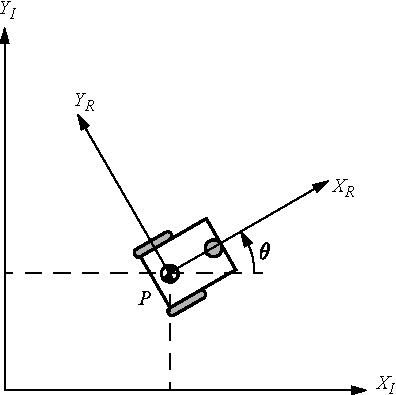
\includegraphics[width=0.3\columnwidth]{./images/coordinate_systems.pdf}
    \end{center}
    Suponga que el sistema de referencia local del robot está alineado de manera que el robot se mueva hacia adelante, como se muestra en la figura.
    
    Primero, considere la contribución de la {\bf velocidad de giro de cada rueda} a la {\bf velocidad de traslación en el punto $\point$} en dirección $+X_{R}$. Si una rueda gira mientras la otra no aporta nada (estacionaria), dado que $\point$ está en el medio entre las dos ruedas, el robot se moverá con la mitad de la velocidad: $\dot{x}_{r1} = \left(\frac{1}{2}\right)r\dot{\varphi}_{1}$ y $ \dot{x}_{r2} = \left(\frac{1}{2}\right)r\dot{\varphi}_{2}$. En un robot de accionamiento diferencial, estas dos contribuciones simplemente se pueden sumar para calcular el componente $\dot{x}_{R}$ de $\dot{\transform{R}{}}$.
\end{frame}

\begin{frame}
    \frametitle{Cinemática de un robot diferencial}
    \footnotesize
    \begin{center}
        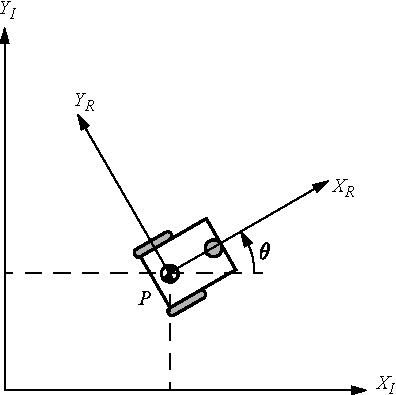
\includegraphics[width=0.3\columnwidth]{./images/coordinate_systems.pdf}
    \end{center}
    
    Pregunta: ¿Qué pasa si cada rueda gira en direcciones opuestas? ¿Cuál es el valor de $\dot{x}_{R}$?
 


    \note{Considere, por ejemplo, un robot diferencial en el que cada rueda gira con la misma velocidad pero en direcciones opuestas. El resultado es un robot giratorio estacionario. Como era de esperar, x_R será cero en este caso.}
    
    El valor de $\dot{y}_{R}$ es aún más sencillo de calcular. Ninguna de las ruedas puede contribuir al movimiento lateral en el marco de referencia del robot, por lo que $\dot{y}_{R}$ es siempre cero.
\end{frame}

\begin{frame}
    \frametitle{Cinemática de un robot diferencial}
    \small

    Finalmente, debemos calcular la componente rotacional $\dot{\theta}_{R}$ de $\dot{\transform{R}{}}$. Una vez más, las contribuciones de cada rueda se pueden calcular de forma independiente y simplemente sumarlas. Considere la rueda derecha (a esta rueda la llamaremos 1). El giro hacia adelante de esta rueda da como resultado una rotación en sentido antihorario en el punto $\point$. Recuerde que si la rueda 1 gira sola, el robot pivota alrededor de la rueda 2. La velocidad de rotación $\omega_{1}$ en $\point$ se puede calcular porque la rueda se mueve instantáneamente a lo largo del arco de un círculo de radio $2l$:

    \begin{equation*}
        \omega_{1} = \dfrac{r\dot{\varphi_{1}}}{2l}
    \end{equation*}

    El mismo cálculo se aplica a la rueda izquierda, con la excepción de que el giro hacia adelante da como resultado una rotación en el sentido de las agujas del reloj en el punto:

    \begin{equation*}
        \omega_{2} = \dfrac{-r\dot{\varphi_{2}}}{2l}
    \end{equation*}
\end{frame}